\chapter{Evaluation}\label{chap:evaluation}
FlyTrap imposes an overhead to vanilla MQTT brokers. It is vital to ensure that added layer of security does not severely impact operation of the broker, as MQTT is a time-sensitive protocol, requiring frequent and rapid responses. In this chapter, I will design experiments to measure latency caused by FlyTrap, operation cost on public blockchain and reflect back to requirements (\& user stories) to ensure that FlyTrap fulfills all of the specified needs

\section{Experimental design}
\subsection{Research question}
I will be looking at evaluation three separate aspects of the implementation and thus can form three research questions, which each of the subsequent sections will attempt to answer:
\begin{enumerate}
  \item  
\end{enumerate}
\subsection{Experiments}
\subsection{Testing environment}
\subsubsection{Hardware}
For tests, virtual machine provided by the University has been used. To ensure that potential noise has been taken into account,  
\subsubsection{Software}
As network latency can be unpredictable and varied, all required software and frameworks have been locally installed in the machine, with FlyTrap communicating via local TCP ports. For TLS encryption, self-signed certificate was also created and provided for FlyTrap. Below you can find a list of specific software used for tests:

\begin{table}[]
\centering
\begin{tabular}{|l|l|}
\hline
\textbf{Software} & \textbf{Version / Implementation}                                        \\ \hline
Blockchain        & Local instance of Geth 1.9.13 running blockchain with Proof-of-Authority \\ \hline
Golang            & Golang 1.13                                                              \\ \hline
MQTT Broker       & Local instance of Mosquitto 1.6.9                                        \\ \hline
\end{tabular}
\end{table}

All source code from the project was compiled into binaries before execution.

\section{Latency Evaluation}
\subsection{Plain TCP}
% \subsubsection{CONNECT}
% \subsubsection{SUBSCRIBE}
% \subsubsection{PUBLISH}

\subsection{With TLS}
% \subsubsection{CONNECT}
% \subsubsection{SUBSCRIBE}
% \subsubsection{PUBLISH}

\section{Cost Evaluation}
As mentioned, Proof-of-Authority networks do not have any currency involved and thus there is no reward for mining. But this removes the benefits of transparency and publicity of the data. On the other hand, running it on a public network (a.k.a. Proof-of-Stake), where miners compete to add new blocks to the network, involves fees and payments.

Six operations performed by FlyTrap were executed a hundred times to extract the average cost in gas. To put those numbers into a perspective, I have also included the equivalent value in USD - assuming relations of 1 ETH = \$182.29 and 1 Gas = 0.0000000054 ETH\footnote{Data from https://ethgasstation.info/ and https://cex.io/eth-usd as of 2020-04-18}

\begin{figure}[h]
    \centering
    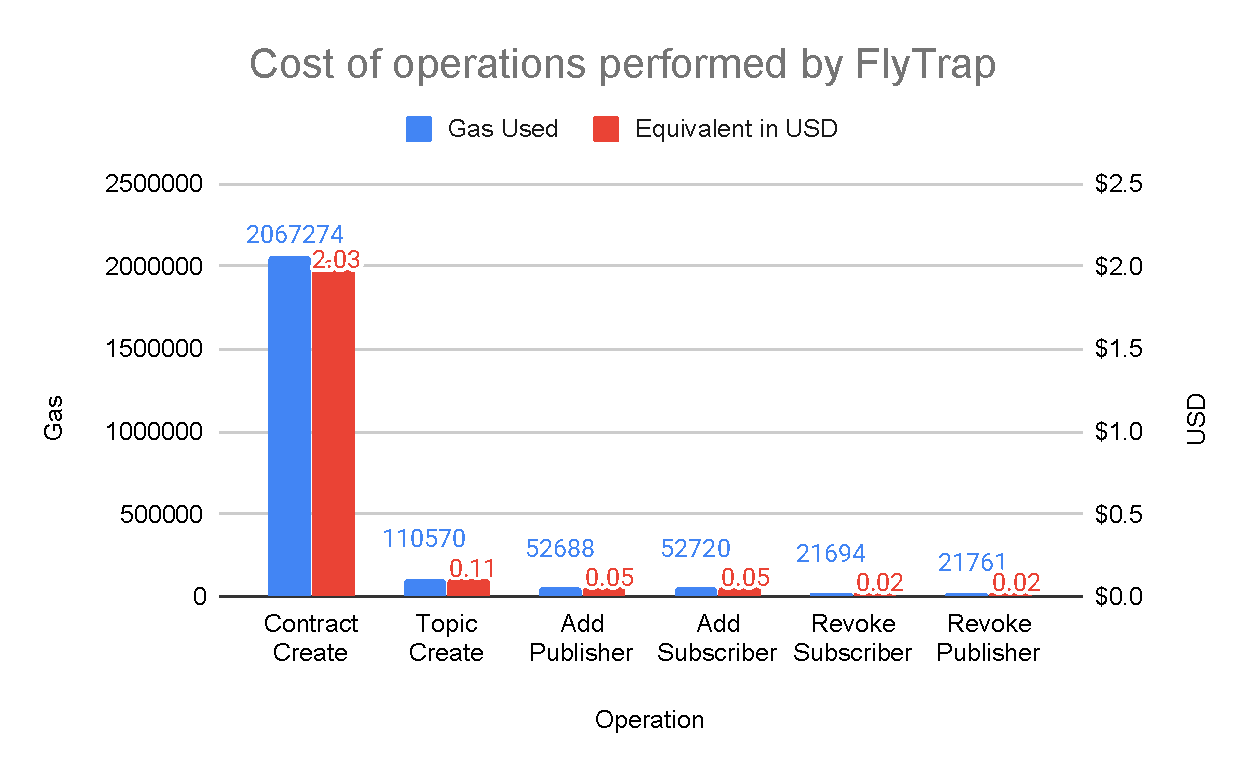
\includegraphics[width=\textwidth]{cost}
    \caption{Comparison of cost of various operations on blockchain}
    \label{fig:cost}
\end{figure}
\subsection{Creating a new contract}
\subsection{Creating a new topic}
\subsection{Adding publisher/subscriber}
\subsection{Summary}

\section{Scenarios Evaluation}
\subsection{Setup}
\subsection{Scenario \#1}
\subsection{Scenario \#2}
\subsection{Scenario \#3}

\section{Results}
